\documentclass[a4paper,12pt]{article}
\usepackage{graphicx,wrapfig}
\usepackage{indentfirst}
\usepackage{amsmath}
\usepackage{algorithm}
\usepackage[margin=1.1in]{geometry}
\usepackage[noend]{algpseudocode}
\usepackage{amssymb}
\usepackage{enumerate}
\usepackage{mathtools}
\usepackage{calligra}
\usepackage{tikz}
\usepackage{tikz,fullpage}

\usetikzlibrary{arrows,%
	arrows.meta,%
	petri,%
	topaths,%
	positioning,%
	quotes}%
\usepackage{tkz-berge}
\usepackage[position=top]{subfig}
\usetikzlibrary {positioning}
\usetikzlibrary{calc}
\captionsetup{labelformat=empty,justification=centering, textfont=normalfont}

\title{ALGORITMICA GRAFURILOR \\
		Tema 3}
\author{Daniș Ciprian\\
		Oloieri Alexandru \\
		Anul II, Grupa A2}
\date{10 ianuarie 2020}

\begin{document}
	
\maketitle

\section{Problema 1}

"$\Rightarrow$": Fie $x$ un e-flux fezabil în rețeaua $R$. Fie $s,t$ două noduri. Avem $G' = (V',E'), V' = V \cup \left\lbrace s,t \right\rbrace, E' = E \cup \left\lbrace si| i \in X \right\rbrace \cup \left\lbrace jt| j \in Y \right\rbrace$ și $c'(si) = 0, i \in X, \linebreak c'(jt) = 0, j \in Y, c'(uv) = c(uv)$.

Considerăm rețeaua elementară $R'(G', s, t, c')$ a.î. $v(x') = v(x), x'(si) = 0, i \in X, x'(jt) = 0,x'(ij) = x(ij), x' : E' \rightarrow \mathbb{R}$ un flux în rețeaua $R'$, și $X,Y \subset V'$. Fie $S',T' \subseteq V'$ a.î. $ S'\cup T' = V',\ S' \cap T' = \emptyset, s \in S', t \in T'$ și $S = S' \setminus \{s\}, T = T' \setminus \{t\}$. 

\begin{itemize}
	\item Avem că $(S',T')$ secțiune în $R' \Rightarrow c'(S',T') \geq v(x') \iff \sum\limits_{i \in S', j \in T'} c'_{ij} \geq \sum\limits_{i \in S', j \in T'} (x'_{ij} - x'_{ji}) \iff \sum\limits_{i \in S, j \in T} c_{ij} \geq \sum\limits_{i \in S', j \in T'} (x'_{ij} - x'_{ji}) (*)$
	\item $\sum\limits_{i \in S', j \in T'} (x'_{ij} - x'_{ji}) = \sum\limits_{i_1 \in S', j_1 \in (T' \cap Y)} (x'_{i_1j_1} - x'_{j_1i_1}) + \sum\limits_{i_2 \in S', j_2 \in (T' \cap X)} (x'_{i_2j_2} - x'_{j_2i_2}) + \linebreak \sum\limits_{i_3 \in S', j_3 \in \left(T' \setminus (X \cup Y)\right)} (x'_{i_3j_3} - x'_{j_3i_3}) \geq \sum\limits_{i_1 \in S', j_1 \in (T' \cap Y)} (x'_{i_1j_1} - x'_{j_1i_1}) + \sum\limits_{i_2 \in S', j_2 \in (T' \cap X)} (x'_{i_2j_2} - x'_{j_2i_2}) = \sum\limits_{i_1 \in S, j_1 \in (T \cap Y)} (x_{i_1j_1} - x_{j_1i_1}) + \sum\limits_{i_2 \in S, j_2 \in (T \cap X)} (x_{i_2j_2} - x_{j_2i_2}) (**)$
	\item $\sum\limits_j x_{ji} - \sum\limits_j x_{ij} \geq - \sigma_i, \forall i \in X$ și $\sum\limits_j x_{ji} - \sum\limits_j x_{ij} \geq \theta_i, \forall i \in Y (***)$
\end{itemize}

Din $(*), (**), (***) \Rightarrow \sum\limits_{i \in S, j \in T} c_{ij} \geq \sum\limits_{j \in (T \cap Y)} \theta_j - \sum\limits_{i \in (T \cap X)} \sigma_i, S,T \subseteq V, S\cup T = V, S \cap T = \emptyset$ (relația are loc pentru $x$ e-flux fezabil în $R(G,X,Y,c)$).
\newline

"$\Leftarrow$": Pentru $\forall S,T \subseteq V$ a.î. $S \cup T = V, S \cap T = \emptyset$, avem că $\sum\limits_{i \in S, j \in T} c_{ij} \geq \sum\limits_{j \in Y \cap T} \theta_j - \sum\limits_{i \in X \cap T} \sigma_i$. 

Pentru orice rețea de transport, există o rețea elementară echivalentă. Fie $R'(G', s, t, c')$ rețeaua de transport elementară echivalentă rețelei $R=(G,X,Y,c)$ din enunț, construită ca mai sus. Existența unui e-flux fezabil în $R'$ ar demonstra și existența unui e-flux fezabil în $R$. Din proprietățile unei rețele de transport reies imediat primele 2 proprietăți ale e-fluxului dintr-o e-rețea: $0 \leq x_{ij} \leq c_{ij}, \forall ij \in E'$ și $\sum\limits_{j}x_{ij} = \sum\limits_{j}x_{ji}, \forall \in V \setminus (X \cup Y)$.


\section{Problema 2}

\subsection{a)}

Descrierea unei rețele de transport ce modelează problema dată presupune descrierea nodurilor din digraf, a arcelor și a capacităților de pe arce din acea rețea.

\begin{itemize}
	\item Nodurile din digraf
	
	Două noduri care trebuie să existe în orice rețea, și care vor face parte și din rețeaua descrisă sunt sursa $s$ și destinația $t$.
	
	Fie \textit{S} = ${S_1,S_2,...,S_p}$ mulțimea studenților; pentru fiecare dintre aceștia vom adăuga câte 3 noduri, noduri pe care le vom grupa în 3 mulțimi: $S_n$ (noduri care vor "uni" studenții cu sursa rețelei), $S_s$ (noduri care se vor ocupa de "conexiunea" studenților cu profesorii specializați) și $S_{ns}$ (noduri care se vor ocupa de "conexiunea" studenților cu profesorii nespecializați).
	
	Fie \textit{P} = ${P_1,P_2,...,P_k}$ mulțimea profesorilor; pentru fiecare dintre aceștia vom adăuga câte un nod, iar reuniunea tuturor acestor noduri o vom nota cu $P_n$.
	
	Așadar, mulțimea nodurilor din rețea este $V = \{s,t\} \cup S_n \cup S_s \cup S_{ns} \cup P_n$.
	
	\item Arcele din digraf
	
	Adăugăm o muchie între $s$ și nodurile din mulțimea $S_n$: $M_1 = \{su | u \in S_n \}$.
	
	Adăugăm o muchie între nodurile din mulțimea $P_n$ și $t$: $M_2 = \{vt | v \in P_n\}$.
	
	Adăugăm o muchie, pentru fiecare student, între nodul din mulțimea $S_n$ și nodul din mulțimea $S_s$, respectiv între nodul din mulțimea $S_n$ și nodul din mulțimea $S_{ns}$: $M_3 = \{xy | x = S_{ni}, y = S_{si}\}$, $M_4 = \{xz | x = S_{ni}, z = S_{nsi}\}$.
	
	Fie $P$ mulțimea tuturor profesorilor, $P_i$ mulțimea profesorilor competenți (specializați) în a judeca lucrarea de licență a studentului $S_i$, și $PN_i = P \setminus P_i$. Adăugăm muchii între nodul din mulțimea $S_s$ pentru fiecare student și nodul fiecărui profesor din mulțimea $P_i$, respectiv între nodul din mulțimea $S_{ns}$ pentru fiecare student și nodul fiecărui profesor din mulțimea $NP_i$: $M_5 = \{yq | y = S_{ni}, q \in P_i\}$, $M_6 = \{zw | z = S_{nsi}, w \in NP_i\}$.
	
	Așadar, mulțimea arcelor din rețea este $E = M_1 \cup M_2 \cup M_3 \cup M_4 \cup M_5 \cup M_6$.
	
	\item Capacitățile arcelor din digraf
	
	Arcele din mulțimea $M_1$ vor avea capacitatea $r$: $c(e) = r, \forall e \in M_1$.
	
	Fie $e_i$ arcul dintre nodul profesorului $i$ din mulțimea $P_n$ și $t$, și $n_i$ numărul maxim de echipe de evaluare din care poate face parte profesorul $i$; vom atribui capacități în felul următor: $c(e_i) = n_i, \forall i \in [1, k]$.
	
	Arcele din mulțimea $M_3$ vor avea capacitatea $a$, iar cele din mulțimea $M_4$ vor avea capacitatea $r-a$: $c(e) = a, \forall e \in M_3$, $c(e) = r-a, \forall e \in M_4$ (a $\leq$ r, deci capacitățile sunt pozitive).
	
	Arcele din mulțimile $M_5$ și $M_6$ vor avea capacitătile 1: $c(e) = 1, \forall e \in M_5 \cup M_6$.
	
\end{itemize}

Modelul descris este o rețea de transport întrucât respectă proprietățile unei astfel de rețele: $G = (V, E)$ este un digraf, $V$ conține 2 noduri speciale, $s$ și $t$, iar pentru toate instanțele problemei în care există cel puțin un student și cel puțin un profesor, $d_G^+(s) > 0$ și $d_G^-(t) > 0$ și fiecare arc $e \in E$ are atribuită o capacitate. 

\subsection{b)}

Existența unei soluții pentru această problemă presupune ca valoarea fluxului maxim din rețea să fie egală cu $p \cdot r$.

Motivul este modul în care au fost alese capacitățile: faptul că arcele din mulțimea $M_1$ au capacitatea $r$ garantează că un student nu va putea să prezinte lucrarea unui număr mai mare de $r$ profesori. Dacă într-un nod corespunzător unui student $i$ întră flux $ = r$, atunci din acel nod va trebui și să iasă flux $ =r$, dintre care $a$ va intra în nodul acelui student din mulțimea $S_s$ (să-l notăm cu $n_1$), iar $r - a$ va intra în nodul studentului din mulțimea $S_{ns}$ (să-l notăm cu $n_2$). Nodul $n_1$ este incident cu nodurile profesorilor competenți în a judeca lucrarea studenților $i$, capacitatea de pe aceste arce este $1$ (deci un profesor poate judeca lucrarea o singură dată), deci dacă în $n_1$ intră $a$ flux, va trebui și să iasă $a$ flux, deci să existe $a$ profesori competenți să-i judece lucrarea. Analog, nodul $n_2$ este incident cu nodurile profesorilor ce nu sunt competenți să judece studentului $i$, capacitatea de pe aceste arce este $1$, deci dacă în $n_2$ intră $r-a$ flux, va trebui să iasă $r-a$ flux, deci lucrarea acestuia să fie verificată de $r-a$ profesori specializați. Capacitatea arcelor din mulțimea $M_2$ este egală cu numărul maxim de echipe de evaluare din care poate face parte un profesor, deci nu va exista nici un profesor care să depășească aceste numere. Așadar, dacă pentru fiecare muchie din $M_1$, fluxul = capacitatea = $r$, înseamnă că pentru fiecare student există 2 mulțimi de profesori $PR_1$ (specializați) și $PR_2$ (nespecializați) care să-i judece lucrarea; și toți profesorii participă într-un număr valid de echipe de evaluare, deci instanța problemei are soluție (mulțimile $PR_1$ și $PR_2$ pentru fiecare student pot fi găsite prin verificarea arcelor cu flux = 1 incidente cu nodurile profesorilor). 

\subsection{c)}

Pentru a decide dacă există soluții va trebui să se construiască rețeaua de transport corespunzătoare instanței problemei, apoi va trebui rulat un algoritm ce calculează fluxul maxim într-o rețea, iar la final trebuie verificat dacă fluxul obținut respectă proprietățile ce confirmă existența unei soluții.

\begin{enumerate}
	\item Construirea rețelei de transport
	
	Complexitatea acestui pas este dată de adăugarea arcelor între noduri (întrucât stabilirea capacității pentru un arc poate fi făcută în momentul adăugării acestuia în digraf): adăugarea arcelor din mulțimile $M_1$ și $M_2$ necesită $p$, respectiv $k$ operații, adăugarea arcelor din mulțimile $M_3$ și $M_4$ necesită (în total) $2 \cdot p$ operații, partea mai costisitoare din punct de vedere a timpului de execuție fiind adăugarea în digraf a arcelor din mulțimile $M_5$ și $M_6$: pentru fiecare student trebuie adăugate muchii către nodul fiecărui profesor (muchie care va "pleca" fie din nodul studentului din mulțimea $S_s$, fie din nodul studentului din mulțimea $S_ns$), deci în total va fi nevoie de $p \cdot k$ operații. Complexitatea acestui pas este deci $\mathcal{O}(p \cdot k)$.
	
	\item Calcularea fluxului maxim din rețeaua de transport
	
	După construirea rețelei de transport, trebuie rulat un algoritm ce calculează fluxul maxim, de exemplu Algoritmul Edmonds-Karp (sau orice alt algoritm ce rezolvă această problemă). Numărul de noduri din rețeaua descrisă este $N = 2 + 3 \cdot p + k$, iar numărul de muchii este $M = 3 \cdot p + k + p \cdot k$. Utilizând algoritmul menționat anterior, complexitatea acestui pas este $\mathcal{O}(N \cdot M^2)$
	
	\item Verificarea existenței unei soluții
	
	Acest pas presupune verificarea faptului că toate arcele incidente cu $s$ (sursa) au fluxul $= r$, ceea ce necesită $p$ operații, deci complexitatea acestui pas este $\mathcal{O}(p)$.  
\end{enumerate}

Complexitatea timp necesară pentru a decide dacă există soluții este dată de cel mai complex (din punct de vedere al timpului de execuție) pas dintre cei descriși mai sus, mai exact este $\mathcal{O}(N \cdot M^2), N = 2 + 3 \cdot p + k, M = 3 \cdot p + k + p \cdot k$.

\section{Problema 3}

\subsection{a)}



\begin{wrapfigure}{H}{6.73cm}
\centering
	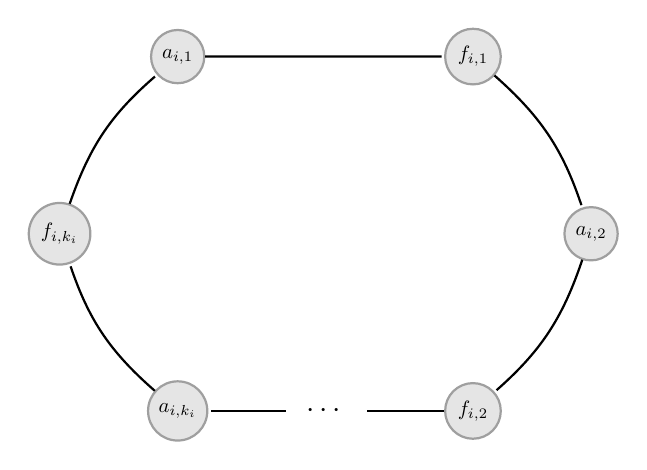
\begin{tikzpicture}[scale = 0.75,transform shape, node distance = 1.5in, on grid, vertex/.style = {circle, draw=gray!75, thick, fill=gray!20, minimum size=1em},edge/.style = {thick, shorten >=1pt}, every edge quotes/.style = {fill=white, font=\Large,inner sep=10pt, anchor=center},bend angle = 15]
	\node[vertex] (0) at (1,6) {$a_{i,1}$};
	\node[vertex] (1) at (6,6) {$f_{i,1}$};
	\node[vertex] (2) at (8,3) {$a_{i,2}$};
	\node[vertex] (3) at (6,0) {$f_{i,2}$};
	\node[vertex] (k-2) at (1,0) {$a_{i,k_i}$};
	\node[vertex] (k-1) at (-1,3) {$f_{i,k_i}$};
	\draw[edge] (0) to (1);
	\draw[edge] (1) to [bend left] (2);
	\draw[edge] (2) to [bend left] (3);
	\draw[edge] (3) edge ["$\cdots$"] ({k-2});
	\draw[edge] ({k-1}) to [bend left] (0);
	\draw[edge] ({k-2}) to [bend left] ({k-1});
	\end{tikzpicture}
\caption{Construcția circuitului $G_i$}
\end{wrapfigure}
{Din $(1) \Rightarrow G_i$ este 2-regulat, $\forall i = \overline{1, n}$. $(*)$ Cum $G_i$ este un circuit de lungime pară $\Rightarrow G_i$ este bipartit. $(**)$ Fie $M_1, M_2 \subset V_i, M_1 = \{a_{i,1},a_{i,2},\dotsc,a_{i,k_i}\}, M_2 =  \{f_{i,1},f_{i,2},\dotsc,f_{i,k_i}\}$ cele 2 partiții ale lui $G_i$ (deduse din construcția lui $G_i$). 

Din $(*), (**) \Rightarrow G_i$ este graf 2-regulat bipartit $\Rightarrow G_i$ admite cuplaj perfect. Fie $Y$ acel cuplaj perfect, $|Y| = |G_i| / 2 = k_i$.

Cum $G_i$ este bipartit și $Y$ cuplaj perfect $\xRightarrow{\text{Konig}}$ pentru $M$ o acoperire minima cu noduri, $\linebreak|M| = |Y| = k_i$. 

Din $(1)$ și $M_1, M_2$ partiții, $|M_1| = |M_2| = k_i, G_i \setminus M_1$ este nul, $G_i \setminus M_2$ este nul (cum $(M_1, M_2)$ bipartiție, avem ca prin eliminarea oricăreia din  submulțimi se șterg toate muchiile) $\Rightarrow M_1, M_2$ acoperiri cu noduri de cardinal minim $k_i$.

Presupunem prin RA că $\exists M'$ o acoperire de cardinal $k_i$, $M' \neq M_1, M' \neq M_2$. Dar din $(1) \Rightarrow |E(G_i \setminus M')| \geq 1 \Rightarrow M'$ nu este acoperire (contradicție) $\Rightarrow$ presupunerea făcută este falsă $\Rightarrow M_1, M_2$ sunt singurele acoperiri de cardinal minim $k_i$ ale lui $G_i, \forall i = \overline{1, n}$.

\subsection{b)}


Următoarele observații ne vor folosi în rezolvarea subpunctelor de mai jos: 
\renewcommand{\theenumi}{\roman{enumi}}
\begin{enumerate}
\item $|G| = \sum\limits_{i=1}^n |V_i| +  \sum\limits_{j=1}^m |W_j| = \sum\limits_{i=1}^n 2k_i +  \sum\limits_{j=1}^m 3 = 3m + 2\cdot \sum\limits_{i=1}^n k_i, V_i \cap W_j = \emptyset, \forall i = \overline{1, n},\linebreak j = \overline{1, m}$

\item Pentru $\forall K_3$, cardinalul unei acoperiri cu noduri $M$ are proprietatea că $2 \leq |M| \leq 3$, întrucât cu un nod putem acoperi exact 2 muchii, iar cele 3 muchii pot fi acoperite de o mulțime de 2 sau 3 noduri.

\item Din a) $\Rightarrow$ cardinalul unei acoperiri cu noduri $M_i$ a lui $G_i, \forall i = \overline{1, n}$ are proprietatea că $k_i \leq |M_i| \leq 2k_i$
\end{enumerate}

\subparagraph{b1)}

Din $U$ acoperă $G$, maniera de construcție a lui $G$ și ii. $\Rightarrow |U \cap W_j| \geq 2, \forall j = \overline{1, m}$.

\subparagraph{b2)}

Din $U$ acoperă $G$, maniera de construcție a lui $G$ și iii. $\Rightarrow |U \cap V_i| \geq k_i, \linebreak \forall i = \overline{1, n} \Rightarrow \left|U \cap \left(\bigcup\limits_{i=1}^n V_i\right)\right| \geq \sum\limits_{i=1}^n k_i, \forall i = \overline{1, n}$. Dar $\sum\limits_{i=1}^n k_i = 3m, \forall i = \overline{1, n}$ ($k_i$ contorizează numărul de apariții ale lui $x_i$ în $\mathcal{C}, \forall i = \overline{1, n}$, $\mathcal{C}$ este format din $m$ clauze, iar fiecare clauză are exact $3$ literali) $\Rightarrow \left|U \cap \left(\bigcup\limits_{i=1}^n V_i\right)\right| \geq 3m, \forall i = \overline{1, n}$.

\subparagraph{b3)}

Din b1) și b2) avem relațiile:
\renewcommand{\labelitemi}{$\ast$}
\begin{itemize}
	\item $\left|U \cap \left(\bigcup\limits_{i=1}^n W_j\right)\right| \geq 2m, \forall j = \overline{1, m}$
	\item $\left|U \cap \left(\bigcup\limits_{i=1}^n V_i\right)\right| \geq 3m, \forall i = \overline{1, n}$
\end{itemize}
Dar din ipoteză avem că $|U| = 5m$, iar din i. că $V_i \cap W_j = \emptyset, \forall i = \overline{1, n}, j = \overline{1, m} \Rightarrow \left|U \cap \left(\bigcup\limits_{i=1}^n W_j\right)\right| = 2m, \forall j = \overline{1, m}$ și $\left|U \cap \left(\bigcup\limits_{i=1}^n V_i\right)\right| = 3m, \forall i = \overline{1, n}$, $\left|U \cap \left(\bigcup\limits_{i=1}^n W_j\right)\right| +  + \left|U \cap \left(\bigcup\limits_{i=1}^n V_i\right)\right| = 5m = |U|\Rightarrow |U \cap W_j| = 2, \forall j = \overline{1, m}, |U \cap V_i| = k_i, \forall i = \overline{1, n}$.

\subparagraph{b4)}

"$\Rightarrow$": $U$ acoperă $G$ și implicit $V_i$. Din b3) $\Rightarrow |U \cap V_i| = k_i$. Acoperirile de cardinal $k_i$ pentru $V_i$ sunt $\{a_{i,1},a_{i,2},\dotsc,a_{i,k_i}\}$, respectiv  $\{f_{i,1},f_{i,2},\dotsc,f_{i,k_i}\}$. Dar $t(x_i) = true$ în $\mathcal{C}$ (ipoteză) $\Rightarrow U \cap V_i = \{a_{i,1},a_{i,2},\dotsc,a_{i,k_i}\}$.

"$\Leftarrow$": Din $U \cap V_i = \{a_{i,1},a_{i,2},\dotsc,a_{i,k_i}\} \Rightarrow U$ acoperă toate aparițiile pozitive ale lui $x_i$ în $\mathcal{C} \Rightarrow t(x_i) = true$ în $\mathcal{C}$.

\subsection{c)}

Din maniera de construcție a lui $U \Rightarrow U \subset V$ și pentru fiecare mulțime de noduri \linebreak $W_j, j = \overline{1, m}, U$ va acoperi exact $2$ noduri, al treilea fiind neapărat adevărat (altfel clauza $C_j$ ar fi falsă, deci și $\mathcal{C}$ ar fi falsă $\rightarrow$ contradicție). Muchia dată de acest al treilea nod și nodul $a_{i,h}$ din mulțimea $V_i$ corespunzătoare, $1 \leq h \leq k_i$ va fi acoperită deoarece $U \cap V_i = \{a_{i,1},a_{i,2},\dotsc,a_{i,k_i}\}$. Prin urmare $\Rightarrow U$ acoperă $G$.

Tot din maniera de construcție a lui $U \Rightarrow |U| = \sum\limits_{j=1}^m 2 + \sum\limits_{i=1}^n k_i = 2m + 3m = 5m \leq k$, unde $k = 5m$.

\section{Problema 4}

\subsection{a)}

Fie $G = (V,E)$ un graf și $c:V \leftarrow \{1, 2, ..., \chi(G)\}$ o $\chi(G)$-colorare a lui $G$.  

O mulțime stabilă maximală este o mulțime de noduri $M$ cu următoarele proprietăți:

\begin{enumerate}
	\item $\forall u, v \in M$, $uv \notin E$ (proprietatea de mulțime stabilă)
	\item $\nexists u \in V$, $u \notin M$ și $M \cup u$ e mulțime stabilă (maximalitatea soluției)
\end{enumerate}

Colorarea $c$ poate fi modificată astfel încât să conțină o clasă de colorare ce este o mulțime stabilă maximală:

Fie $col$ o culoare oarecare, de exemplu $1$, și $MS$ mulțimea stabilă corespunzătoare clasei de colorare $col$. Ne vom baza pe următoarea observație: orice nod care nu face parte dintr-o clasă de colorare este adiacent cu cel puțin un nod din acea clasă de colorare. Așadar, cât timp mai există noduri $u$ astfel încât $c(u) \neq col$ și $u$ nu e adiacent cu vreun nod $v$, $v \in MS$, putem colora nodul $u$ cu culoarea $col$ ($c(u)=col$). În final, colorarea este în continuare validă (datorită condițiilor impuse pentru a colora un nod $u$ cu col), $MS$ este de cardinal maxim (dacă nu ar fi așa, am mai putea efectua un pas al operației descrise) iar numărul cromatic al grafului $G$ a rămas același. Acesta nu ar fi putut să crească (nu am adăugat culori noi), însă nici să scadă (adică să dispară o clasă de colorare) întrucât asta ar fi contrazis optimalitatea colorării inițiale $c$. 

Deci pentru orice graf există o $\chi(G)$ colorare cu proprietatea că cel puțin una dintre clasele de colorare este mulțime stabilă maximală, colorare ce poate fi "construită" dintr-o colorare optimală oarecare.

\subsection{b)}

Fie $G = (V,E)$ un graf, $c:V \leftarrow \{1, 2, ..., \chi(G)\}$ o $\chi(G)$ colorare a lui $G$ și $x$ și $y$ două noduri neadiacente. Distingem două cazuri:

\subsubsection{$c(x) \neq c(y)$}

Fie graful $G_2 = (V, E \cup \{xy\})$. Cum $x$ și $y$ sunt în clase stabile diferite în colorarea $c$, adăugarea muchiei $xy$ nu va modifica proprietatea de submulțime stabilă a niciunei clase de colorare, deci $\chi(G)$ nu poate crește, ceea ce implică faptul că $\chi(G_2) \leq \chi(G)$, însă $\chi(G_2)$ nu poate fi mai mic decât $\chi(G)$, deci $\chi(G) = \chi(G_2)$.

Fie graful $G_3 = G|xy$. $\chi(G_3)$ nu poate fi mai mic decât $\chi(G)$ pentru că altfel am putea decontracta perechea $(x,y)$ din $G_3$ și am obține că graful $G$ are un număr cromatic mai mic decât $\chi(G)$, care este deja minim posibil, așadar $\chi(G_3) \geq \chi(G)$, întrucât există grafuri pentru care concatenarea perechii $(x,y)$ să ducă la creșterea numărului cromatic, de exemplu:

\begin{wrapfigure}{H}{6.73cm}
	\centering
	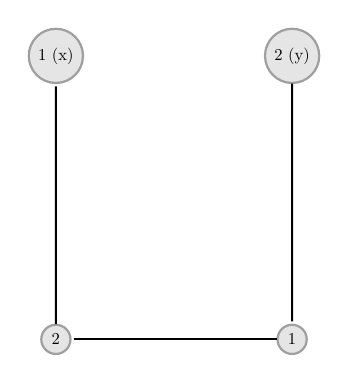
\begin{tikzpicture}[scale = 0.6,transform shape, node distance = 1.5in, on grid, vertex/.style = {circle, draw=gray!75, thick, fill=gray!20, minimum size=1em},edge/.style = {thick, shorten >=1pt}, every edge quotes/.style = {fill=white, font=\Large,inner sep=10pt, anchor=center},bend angle = 15]
	\node[vertex] (0) at (1,6) {1 (x)};
	\node[vertex] (1) at (6,6) {2 (y)};
	\node[vertex] (2) at (6,0) {1};
	\node[vertex] (3) at (1,0) {2};
	\draw[edge] (3) to (0);
	\draw[edge] (2) to (3);
	\draw[edge] (1) to (2);
	\end{tikzpicture}
\end{wrapfigure}

Graful din imagine este bipartit, 2 culori fiind suficiente pentru a-l colora, însă dacă nodurile $x$ și $y$ ar fi contractate, graful ar deveni $K3$, fiind necesare 3 culori.

\subsubsection{$c(x) = c(y)$}

Pentru graful $G_3$, contractarea perechii $(x,y)$ nu a avut nici un efect asupra numărului cromatic: cum $c(x)=c(y)$, iar $x$ și $y$ erau adiacente în $G$ numai cu noduri $u$ ce au proprietatea: $c(u) \neq c(x)$, $c(u) \neq c(y)$, nu e nevoie să adăugăm culori noi, deci $\chi(G_3)=\chi(G)$.

În graful $G_2$ în schimb, adăugarea muchiei $xy$ va impune schimbarea uneia dintre valorile $c(x)$ sau $c(y)$ (pentru a avea o colorare validă a grafului), deci $\chi(G_2) \geq \chi(G)$.
\newline

Din \textbf{4.2.1} $\Rightarrow$ dacă $\chi(G_3) > \chi(G)$, atunci $\chi(G) = \chi(G_2)$ (1).

Din \textbf{4.2.2} $\Rightarrow$ dacă $\chi(G_2) > \chi(G)$, atunci $\chi(G) = \chi(G_3)$ (2).

Din \textbf{(1)} și \textbf{(2)} $\Rightarrow$ $\chi(G) = min\{\chi(G_2), \chi(G_3)\} = min\{\chi(G+xy), \chi(G|xy)\}$.

\end{document}